\documentclass[sans]{beamer}

% \usetheme{Boadilla}
\mode<presentation>
{
	% \usetheme{CambridgeUS}
	\usetheme{Hannover}
	% \usetheme{Bergen}
	\usecolortheme{whale}
	% \usefonttheme{serif}
	% \usefonttheme{professionalfonts}
	% \usefonttheme{structureitalicserif}
}

\usepackage{cmap}
\usepackage{listings}
\usepackage{lmodern}
\usepackage{color}
\usepackage{minted}
\usepackage{graphicx}
\usepackage{tikz}
\usepackage{wrapfig}

% \usepackage[labelformat=empty]{subcaption}
\usepackage[labelformat=empty]{caption}

% \usefonttheme{professionalfonts} % using non standard fonts for beamer
% \usefonttheme{sansserif} % default family is serif
% \usepackage{fontspec}
% \usepackage[T2A]{fontenc}
% \setmainfont{Comic Sans MS}

% \usepackage[utf8]{inputenc}
% \usepackage[russian]{babel}

\usepackage{fontspec}
% \setmainfont[Mapping=tex-text]{CMU Serif}



\usepackage{polyglossia}
\setdefaultlanguage{russian}

% \newfontfamily\cyrillicfont[Script=Cyrillic]{Comic Sans MS}
% \newfontfamily{\cyrillicfontt} {Comic Sans MS}
% \newfontfamily{\cyrillicfonttt}{Comic Sans MS}

\setmainfont[Ligatures=TeX]{DejaVu Serif}
\setsansfont[Ligatures=TeX]{DejaVu Sans}
% \setmainfont[Ligatures=TeX]{Comic Sans MS}
% \setsansfont[Ligatures=TeX]{Comic Sans MS}
\setmonofont{DejaVu Sans Mono}

% \setmathfont{XITS Math}
% \defaultfontfeatures{Scale=MatchLowercase,Mapping=tex-text}

\begin{document}

\title[XQuery/XUpdate]{XQuery/XUpdate}

\institute{SE, SPbSU}

\author
[Podkopaev Anton]{Podkopaev Anton, \texttt podkoav239@gmail.com}
\date [07-10-13]{07 October 2013}

\begin{frame}[plain]
	\titlepage
\end{frame}

\section{XQuery}

\begin{frame}{What is XQuery?}
	\begin{columns}
		\begin{column}{0.4\linewidth}
			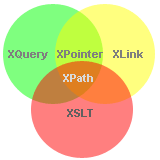
\includegraphics[width = \linewidth]{images/xpath.png}
		\end{column}

		\begin{column}{0.5\linewidth}
			\begin{itemize}
				\item The language for querying XML data
				\item For XML like SQL for databases
				\item Built on XPath expressions
				\item Supported by all major databases
				\item A W3C Recommendation
			\end{itemize}
		\end{column}
	\end{columns}
\end{frame}

\begin{frame}{XPath}
	A query language for selecting nodes from an XML document
	\begin{block}{Example XMLs}
		\inputminted[fontsize=\tiny]{xml}{codes/ex24.xml}
	\end{block}
	\begin{block}{Query examples}
		\inputminted[fontsize=\tiny]{xquery}{codes/ex25.xml}
	\end{block}
\end{frame}

\begin{frame}{XQuery and XPath}
	XQuery 1.0 and XPath 2.0 share the same data model and support the same functions and operators

	% Может быть тут написать про XSLT
\end{frame}

% XSLT functionalities overlap with those of XQuery, which was initially conceived as a query language for large collections of XML documents

 % XSLT was primarily conceived as a stylesheet language whose primary goal was to render XML for the human reader on screen, on the web (as web template language), or on paper

% XQuery was primarily conceived as a database query language in the tradition of SQL

\begin{frame}{XSLT}
	\begin{itemize}
		\item eXtensible Stylesheet Language Transformations
		\item Turing-complete language
		\item Conceived as a stylesheet language whose goal was to render XML for the human reader
	\end{itemize}
\end{frame}

% \begin{frame}{Example}
% 	\inputminted{xquery}{codes/ex1.xq}
% \end{frame}

\begin{frame}{XQuery. Usages}
	\begin{itemize}
		\item Extract information to use in a Web Service
		\item Generate summary reports
		\item Transform XML data to XHTML
		\item Search Web documents for relevant information
	\end{itemize}
\end{frame}

\begin{frame}{XML example}
	\begin{columns}
		\begin{column}{0.45\linewidth}
			\inputminted[fontsize=\tiny]{xml}{codes/ex2.xml}
		\end{column}
		\begin{column}{0.55\linewidth}
			% \begin{block}{Query example}
			\begin{itemize}
				\item \inputminted[fontsize=\tiny]{xquery}{codes/ex3.xq}
				\item \inputminted[fontsize=\tiny]{xquery}{codes/ex4.xq}
			\end{itemize}
			% \end{block}
		\end{column}
	\end{columns}
\end{frame}

\begin{frame}{FLWOR Expressions}
	For, Let, Where, Order by, Return

	\vspace{1cm}

	\begin{block}{Example}
		\inputminted{xquery}{codes/ex5.xq}
	\end{block}
\end{frame}

\begin{frame}{FLWOR + HTML}
	\begin{block}{Script}
		\inputminted[fontsize=\footnotesize]{xquery}{codes/ex6.html}
	\end{block}

	\begin{block}{Result}
		\inputminted[fontsize=\footnotesize]{html}{codes/ex7.html}
	\end{block}
\end{frame}

\begin{frame}{Custom functions}
	\begin{block}{Syntax}
		\inputminted[fontsize=\tiny]{xquery}{codes/ex8.xq}
	\end{block}
	\begin{block}{Example}
		\inputminted[fontsize=\tiny]{xquery}{codes/ex9.xq}
	\end{block}
\end{frame}

% XML may be strongly typed and governed by a W3C XML Schema, and a strongly typed query language with static typing can prevent many errors for this kind of data.

% XML may be governed by another schema language, such as DTDs or RELAX-NG.

% XML may have an ad hoc structure and no schema, and the whole reason for performing a query may be to discover the structure found in a document. For this kind of data, the query language should be able to process whatever data exists, with no preconceived notions of what should be there.

% XML may be used as a view of another system, such as a relational database. These systems are typically strongly typed, but do not use W3C XML Schema as the basis for their type system. Fortunately, standard mappings are emerging for some systems, such as SQL's mappings from relational schemas to W3C XML Schema. These are defined in the SQL/XML proposal, which provides standard XML extensions to SQL [SQLXML].

% XML data sources may have very complex structure, and expressions in XQuery must be well defined in terms of all the structures to which the operands can evaluate.

\subsection{Data Types}

\begin{frame}{Data Types}
	\begin{itemize}
		\item XML may be strongly typed and governed by a W3C XML Schema
		\item XML may be governed by another schema language
		\item XML may have an ad hoc structure and no schema
		\item XML may be used as a view of another system, such as a relational database
		\item XML data sources may have very complex structure
	\end{itemize}

	\begin{block}{}
		XQuery allows queries that rely on very little type information or take advantage of type information to detect potential errors before a query is ever executed
	\end{block}

\end{frame}

% The type system of XQuery is based on [SCHEMA]. There are two sets of types in XQuery: the built-in types that are available in any query, and types imported into a query from a specific schema. 

\begin{frame}{Example}
	\begin{block}{Without types}
		\inputminted[fontsize=\tiny]{xquery}{codes/ex26.xq}
	\end{block}
	\pause
	\begin{block}{Declaration with types}
		\inputminted[fontsize=\tiny]{xquery}{codes/ex27.xq}
	\end{block}
	\pause
	\begin{block}{Type error}
		\inputminted[fontsize=\tiny]{xquery}{codes/ex28.xq}
	\end{block}
\end{frame}

\begin{frame}{Data Types}
	Shares the same data types as XML Schema 1.0 (XSD)

	\begin{itemize}
		\item String
			\begin{itemize}
				\item NormalizedString
				\item Token
				\item ...
			\end{itemize}
		\item Date
		\item Numeric
			\begin{itemize}
				\item Decimal
				\item Integer
				\item ...
			\end{itemize}
		\item Misc
			\begin{itemize}
				\item Boolean
				\item Binary
				\item AnyURI
				\item ...
			\end{itemize}
	\end{itemize}
\end{frame}

\subsection{JSON}

\begin{frame}{JSON}
	\begin{itemize}
		\item JSONiq
		\item XQuery 3.1

		\color{blue} \url{w3.org/blog/2013/09/xml-json-xslt-and-xquery/} \color{black}
	\end{itemize}
\end{frame}

% \begin{frame}{Features}
% 	\begin{itemize}
% 		\item Case-sensitive
% 		\item Conditional expressions
% 		\item Custom functions
% 	\end{itemize}
% \end{frame}

\section{XUpdate}

% \begin{frame}{What is XUpdate?}
% 	\begin{itemize}
% 		\item A lightweight XML query language for modifying XML data
% 		\item For users not content to wait for the XQuery Update Facility extension of the W3C standard
% 		\item Last Working Draft, September 14, 2000
% 	\end{itemize}
% \end{frame}

\begin{frame}{What is XUpdate?}
	\begin{itemize}
		\item Makes extensive use of the expression language defined by XPath for selecting elements for updating and for conditional processing
		\item A pure descriptive language which is designed with references to the definition of XSL Transformations
		\item Has found a niche market of users not content to wait for the XQuery Update Facility
	\end{itemize}
\end{frame}

\begin{frame}{Modifications}
	\begin{block}{xupdate:modifications}
	\begin{itemize}
		\item xupdate:insert-before
		\item xupdate:insert-after
		\item xupdate:append
		\item xupdate:update
		\item xupdate:remove
		\item xupdate:rename
		\item xupdate:variable
		\item xupdate:value-of
		\item xupdate:if
	\end{itemize}
	\end{block}
\end{frame}

\begin{frame}{Insertion}
	\begin{block}{Commands}
	\begin{itemize}
		\item xupdate:insert-before
		\item xupdate:insert-after
	\end{itemize}
	\end{block}

	\begin{block}{Element types}
	\begin{itemize}
		\item xupdate:element
		\item xupdate:attribute
		\item xupdate:text
		\item xupdate:processing-instruction
		\item xupdate:comment
	\end{itemize}
	\end{block}
\end{frame}

\begin{frame}{Insertion. Element}
	\begin{block}{Code}
		\inputminted[fontsize=\footnotesize]{xml}{codes/ex10.xml}
	\end{block}
	\begin{block}{Result}
		\inputminted[fontsize=\footnotesize]{xml}{codes/ex11.xml}
	\end{block}
\end{frame}

\begin{frame}{Insertion. Attribute}
	\begin{block}{Code}
		\inputminted[fontsize=\tiny]{xml}{codes/ex12.xml}
	\end{block}
	\begin{block}{Result}
		\inputminted[fontsize=\footnotesize]{xml}{codes/ex13.xml}
	\end{block}
\end{frame}

% TODO: Read about processing-instructions

\begin{frame}{Append}
	\begin{block}{Element types}
	\begin{itemize}
		\item xupdate:element
		\item xupdate:attribute
		\item xupdate:text
		\item xupdate:processing-instruction
		\item xupdate:comment
	\end{itemize}
	\end{block}

	\begin{block}{Position}
		The optional child attribute specifies the position of the newly appended child node
	\end{block}
\end{frame}

\begin{frame}{Append. Example}
	\begin{block}{Code}
		\inputminted[fontsize=\footnotesize]{xml}{codes/ex14.xml}
	\end{block}
	\begin{block}{Result}
		\inputminted[fontsize=\footnotesize]{xml}{codes/ex15.xml}
	\end{block}	
\end{frame}

\begin{frame}{Update}
	\begin{block}{Code}
		\inputminted[fontsize=\footnotesize]{xml}{codes/ex16.xml}
	\end{block}
	\begin{block}{Result}
		\inputminted[fontsize=\footnotesize]{xml}{codes/ex17.xml}
	\end{block}
\end{frame}

\begin{frame}{Remove}
	\begin{block}{Code}
		\inputminted[fontsize=\footnotesize]{xml}{codes/ex18.xml}
	\end{block}
	\begin{block}{Result}
		\inputminted[fontsize=\footnotesize]{xml}{codes/ex19.xml}
	\end{block}		
\end{frame}

\begin{frame}{Rename}
	\begin{block}{Code}
		\inputminted[fontsize=\footnotesize]{xml}{codes/ex20.xml}
	\end{block}
	\begin{block}{Result}
		\inputminted[fontsize=\footnotesize]{xml}{codes/ex21.xml}
	\end{block}		
\end{frame}

\begin{frame}{Variables}
	\begin{block}{With variable}
		\inputminted[fontsize=\tiny]{xml}{codes/ex22.xml}
	\end{block}
	\begin{block}{With variable}
		\inputminted[fontsize=\tiny]{xml}{codes/ex23.xml}
	\end{block}		
\end{frame}

\begin{frame}{Realizations}
	\begin{itemize}
		\item Xmldiff
		% Xmldiff is a Python tool that figures out the differences between two similar XML files, in the same way the diff utility does it for text files. Xmldiff can produce an XUpdate output
		\item 4Suite
		% 4Suite is a collection of Python tools for XML processing and object database management that also implements an XUpdate command line interface
		\item Lexus
		% Lexus is a Java based XUpdate implementation. Lexus is used in several Open Source projects: Ozone, Xindice
		\item Jaxup
		% Jaxup is an XML update engine written in Java to work against a variety of XML based object models such as DOM, dom4j and JDOM. It supports the XUpdate standard draft and will support other xml update standards as they become available
	\end{itemize}
\end{frame}

\end{document}